\section{Applications Part One - Railroads}

So while working on this topic, I kept thinking to myself: What practical applications does this theory have out in the real world? Where in science/nature/technology do we spot $N$-Units Away Curves? The first immediate thought that comes to my mind is railroad tracks.

The left rail of a railroad track is set to be exactly the same consistent distance away from the right rail at all locations. You literally have two curves that remain some fixed $N$-Units Away from one another at all spots! This is what lets a train of fixed width ride along it smoothly.

So considering that my $N$-Units Away Theory is brand new and yet trains have been driving on tracks since the early 1800's, I was instantly stuck with the question: How is it that railroad engineers have been building fairly spot on approximations of $N$-Units Away Curves for all these years?

I did some significant research into the topic, assisted greatly by a book I found called \textit{Railroad Engineering} by William W. Hay, and discovered the truly improbable, ridiculous, and highly enjoyable answer. When railroad engineers first want to lay down a railroad track through a new area, first they prepare a track bed for the train. Sometimes this means digging a trench for a train track. More often it just means clearing away debris / trees and making the ground level along the desired route. Next they unload 60 foot long prefabricated track pieces (the underlying supportive cross beams that the rails will sit atop). Finally they lay down long long bendy rail strips on top made of a high quality steel alloy. They place these rail strips down onto the cross beams sorta any which way. The distance between them at this stage doesn't really matter. They’re all higgledy-piggledy. It’s the furthest thing from a nice approximation of $N$-Units Away Curves. How do they then get from that to the nice $N$-Units Away Curves-like final product?

They use an amazing device called a Rail Threader! It operates like a gigantic zipper. It has highly flexible wheels and can roll along the highly unevenly distant-from-each-other rails. Periodically it pauses, puts down two large hydrolic ``feet'' and lifts off the ground, taking the flexible rails with it about a foot into the air. It then moves them laterally to the exact desired standard gauge distance the rails should be from one another and places them down. We now have a beautiful approximation of an $N$-Units Away Curve which the railroad crews then bolt down into place. The Rail Threader acts like a zipper, taking in the higgledy-piggledy rails and leaving behind it as it goes a nice perfect Standard-Gauge N-Units Away Curves track. Absolutely amazing! A real ``engineer's answer'' to an otherwise very tricky math problem.

\renewcommand\w{0.3\linewidth}
\renewcommand\fw{0.9\textwidth}

\begin{figure}[h]
  \centering
  \begin{minipage}[b]{\w}
    \centering
    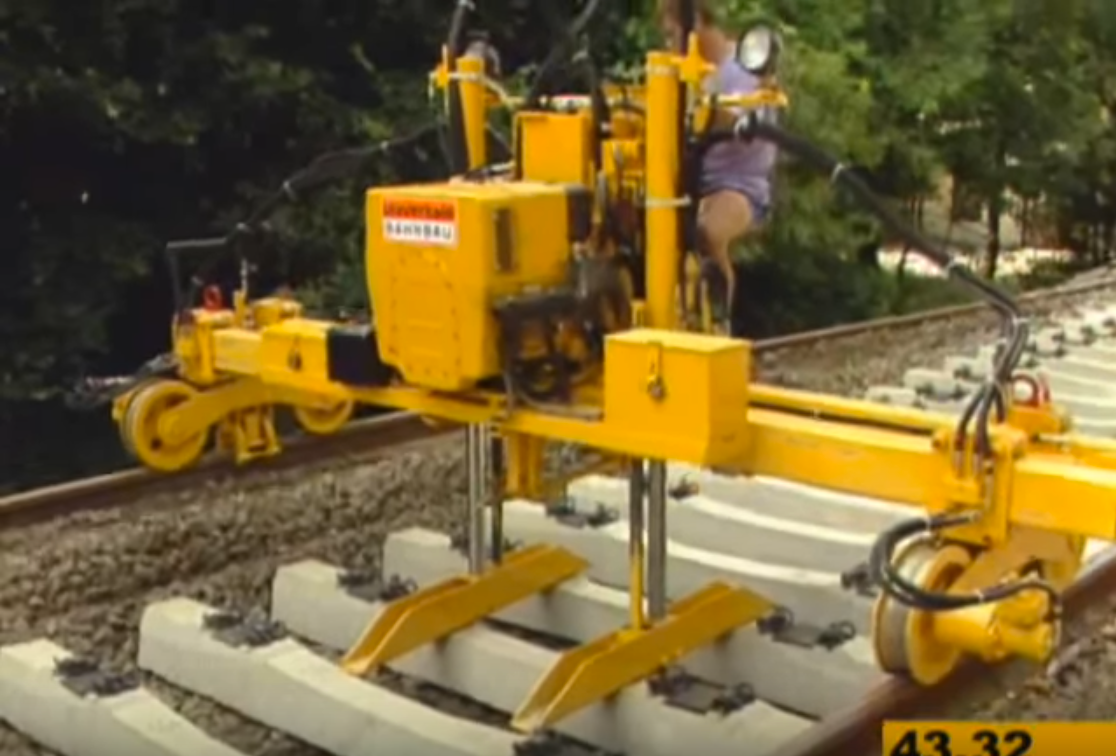
\includegraphics[width=\fw]{img/13-app/01.png}
    \caption{Caption}
    \vspace{4ex}
  \end{minipage} % end
  \begin{minipage}[b]{\w}
    \centering
    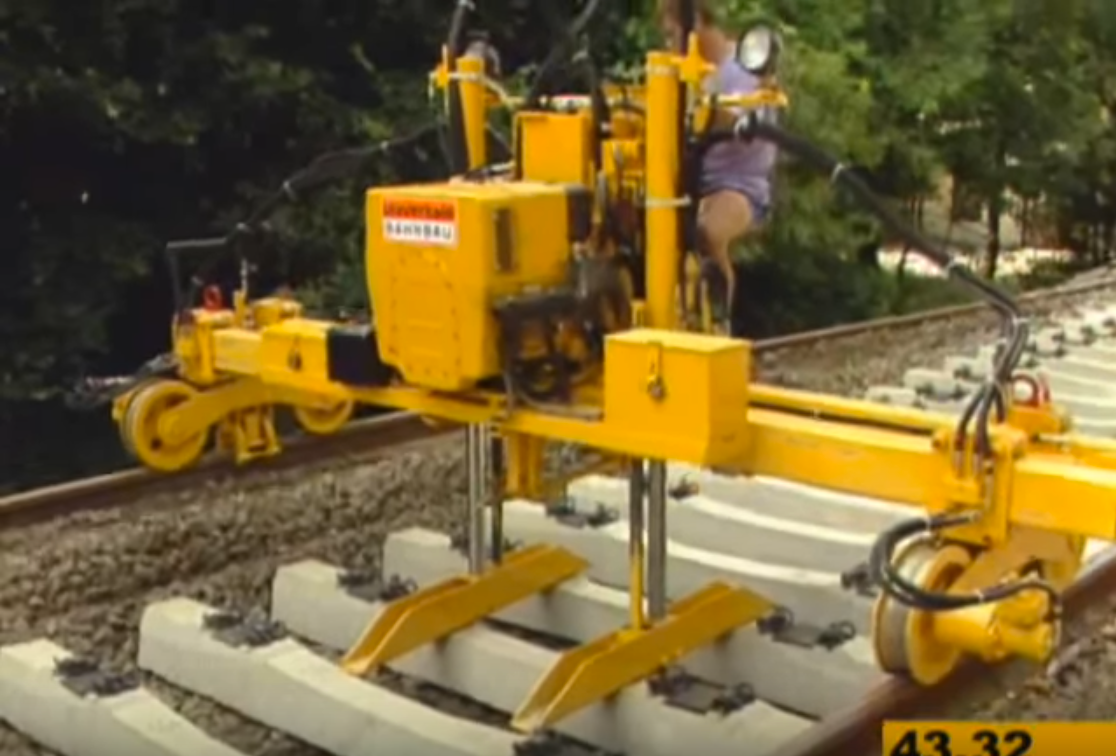
\includegraphics[width=\fw]{img/13-app/02.png}
    \caption{Caption}
    \vspace{4ex}
  \end{minipage} % end
  \begin{minipage}[b]{\w}
    \centering
    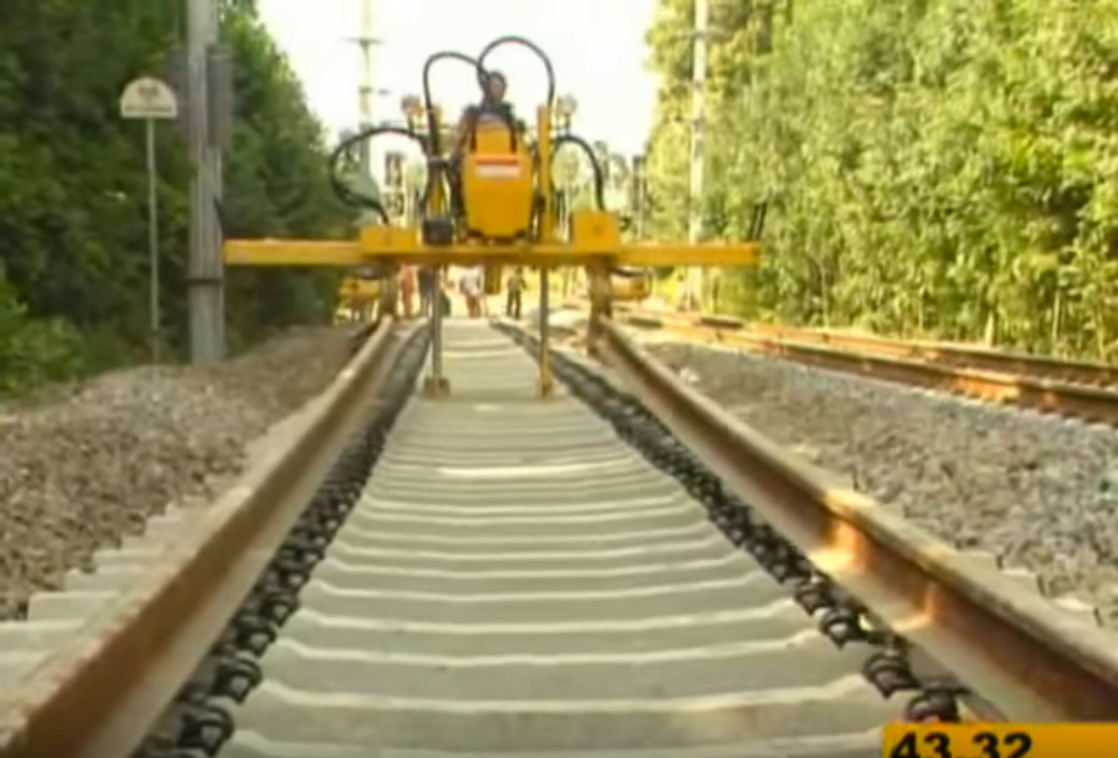
\includegraphics[width=\fw]{img/13-app/03.png}
    \caption{Caption}
    \vspace{4ex}
  \end{minipage} % end
\end{figure}
